\section{Shower Reconstruction}
\label{sec:reco}

In this section we describe the underlying concepts for shower reconstruction.
The technical details are dispicted in DocDB ?.

% -----------------------------------------------------------------------
\subsection{Brief Introduction to Pandora}
\label{sec:pandora}

Pandora~\cite{DocDB5828} is a toolkit for pattern recognition, aiming to 
reconstruct particle flow in detectors with fine granularity, such as
detectors of high-energy lepton colliders, and LAr TPC.
MicroBooNE uses Pandora, which is integrated into the LArSoft toolkit
via the \texttt{larpandora} interface,
as one of the pattern recognition and clustering algorithms. \\
\\
% Concept of PFParticle
The outputs of Pandora are centralized in particle-flow particles, 
or PFParticles, which include,
\begin{itemize}
\item PDG code: mainly four types, 11 (shower-like),
      13 (track-like), 12 (neutrino-like PFParticle with a shower-like
      daughter), and 14 (neutrino-like PFParticle with all daughters
      track-like).
\item Parent: indicates the parent of the PFParticle.
\item Daughters: indicates the daughters (possibly a plural number) of
      the PFParticle.
\end{itemize}
Further, the PFParticles associate to the following objects created
by Pandora,
\begin{itemize}
\item Cluster: collection of hits from a separate hit finding algorithm.
\item Spacepoint: three-dimensional points indicating the 3D positions
      of charge deposition; associating to the two-dimensional hits
      reconstructed by the hit finder.
\item Vertex: a 3D point representing the starting point of the PFParticle.
\item Seed: not generated in a shower-like PFParticle
\item Track
\end{itemize}

In this study, each PFParticle is exploited as a shower candidate.
We describe the algorithms of shower reconstruction 
utilizing PFParticles and associated features in the following sections.

% -----------------------------------------------------------------------
\subsection{Direction}
\label{sec:shr_direction}

An important variable from shower reconstruction is the direction of the 
original electromagnetic particle.
We assume the vectorial summation of all showering particles 
would retain the direction of the original particle.
To obtain the direction,
we simply perform a 3-dimensional (3D) principal component 
analysis (PCA) over all the spacepoints associated to a PFParticle.
The eigenvector corresponding to the largest eigenvalue determined by
PCA is taken to be the direction of the shower, as it represents the axis
with the largest possible variance of the distribution of the spacepoints.
The forward or backward direction is determined from the ordering of
the spacepoints, which is reconstructed based on the particle flow approach
within the Pandora toolkit.\\
% It will be revisited in the succeeding
% shower reconstruction algorithms.\\
\\
In addtion, the (unweighted) 3D centroid of a PFParticle evaluated
by PCA is saved for possible exploitation in other algorithms.

% -----------------------------------------------------------------------
\subsection{Geometry}
\label{sec:shr_geometry}

% Length, width
The length and the 2D width of a shower is also determined by the same
principal component analysis.
As the largest eigenvalue of the PCA accounts for the possible largest
variance of the spacepoint distribution, the distance of three
standard deviations can be used to represent the length of a shower.
Moreover, the eigenvalues, or the variances, from PCA determine semi-axes
of the spacepoint distribution, and therefore a factor of two has to be
applied to obtain the full shower length.
\begin{equation}
\label{eq:shrlength}
\textrm{Shower Length} = 2\times 3\times \sqrt{\textrm{the largest eigenvalue from PCA}}
\end{equation}
Similarly, we use~\Cref{eq:shrlength} with the other two eigenvalues
from PCA to dispict the width of a shower.
Currently the widths in the plane orthogonal to the principal component
axis are not combined but stored individually.\\
\\
% Opening angle
The opening angle of a shower can also simply approximated using the
eigenvalues of PCA.
A straightforward approach is to interpret the tangent of half the 
opening angle as the ratio of the standard deviations for the second
largest eigenvalue to that for the largest one, i.e.
\begin{equation}
\label{eq:shropeningangle}
\textrm{Opening Angle} = 2\times \tan^{-1}({\frac{\textrm{the 2nd largest eigenvalue}}{\textrm{the largest eigenvalue}}})
\end{equation}

% -----------------------------------------------------------------------
\subsection{Starting Point}
\label{sec:shr_startingpt}

The starting point of a shower is determined by the vertex associated to
the PFParticle.
Both the vertex and the association are reconstructed by the algorithms
within Pandora.\\
\\
An example of a reconstructed shower in a single electron simulated event
is illustrated in~\Cref{fig:shr_reco_example}.
The cone represnts the location and the geometry of the shower, and
the tip of the cone indicates the starting point discussed in this section.

% -----------------------------------------------------------------------
\begin{figure}[htbp]
\begin{center}
\begin{subfigure}{0.45\textwidth}
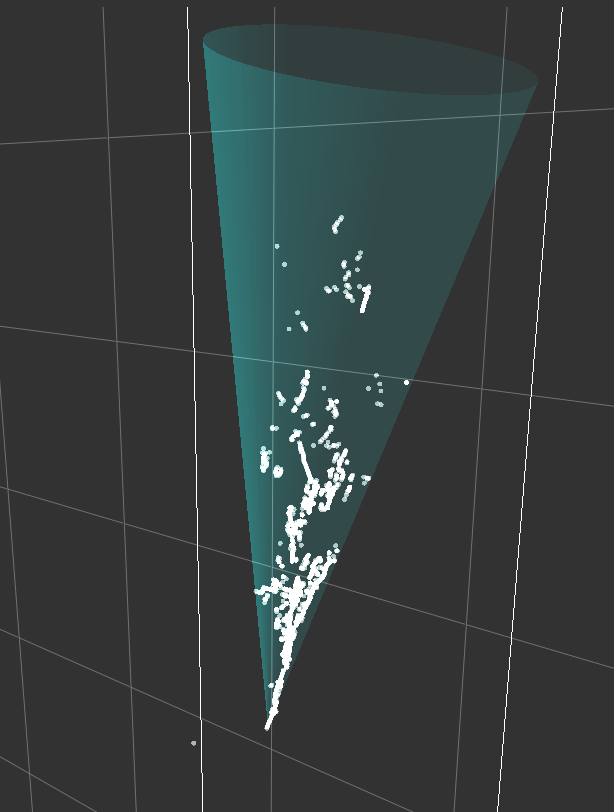
\includegraphics[angle=270,width=\linewidth]{figs/reco/single_e_Evt1.png}
\caption{Reconstructed shower in 3D event display.
The points indicate the reconstructed spacepoints, and the cone
represents the shower.}
\label{fig:shr_reco_example_3d}
\end{subfigure}
\begin{subfigure}{0.45\textwidth}
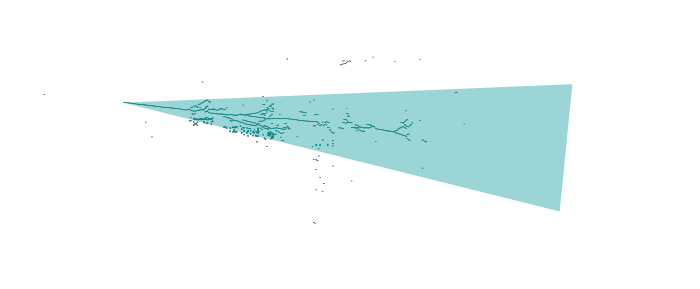
\includegraphics[width=0.85\linewidth]{figs/reco/single_e_Evt1U.png}\\
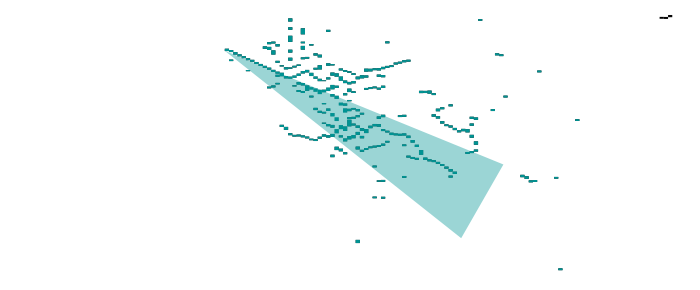
\includegraphics[width=0.85\linewidth]{figs/reco/single_e_Evt1V.png}\\
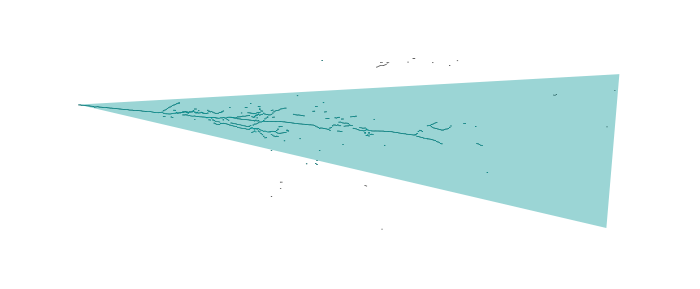
\includegraphics[width=0.85\linewidth]{figs/reco/single_e_Evt1Y.png}
\caption{Reconstructed shower in the U, V, and Y wire planes.
The points represent the reconstructed hits, while the triangles
profile the reconstructed shower.}
\label{fig:shr_reco_example_2d}
\end{subfigure}
\caption{An example of a reconstructed shower from single electron
simulated event.}
\label{fig:shr_reco_example}
\end{center}
\end{figure}
% -----------------------------------------------------------------------

% -----------------------------------------------------------------------
\subsection{Calorimetry}
\label{sec:shr_calorimetry}

The calorimetry quantities, such as energy, dQ/dx, and dE/dx, are
evaluated using the algorithms described in DocDB XXXX.
The sources of discrepancy in these quantities between the other
shower reconstruction chain and this work are listed below,
\begin{itemize}
\item Clustering: Pandora provides the input clusters for energy
      evaluation, and the reconstructed energy obviously depends
      on clustering efficiency.
\item Shower direction: The reconstructed dQ/dx and dE/dx rely on
      both energy and shower direction.  
      The different clustering (i.e. the  choice of hits) and 
      shower direction thereby would alter the values of such
      quantities.
\end{itemize}

The calorimetry quantities are evaluated for each individual plane,
since the charge and energy variables are determined from charge
deposition in hits, 2D reconstructed objects.

